\chapter{Probability and Statistics: Studying Uncertainty Precisely}

\section{A Birthday Bet}

At the start of term, several new pupils join a class, bringing its total to thirty. During break, someone suggests a game: everyone announces their birthday, month and day only, to see whether any two match. Class representative Xiaolin confidently says, ``There are three hundred and sixty-five days and only thirty of us. A match is far too unlikely. I bet there won't be one!'' His deskmate Xiaoyu smiles: ``I'd bet there probably will. A bottle of fizzy drink?''

The pupils start announcing birthdays. Somewhere in the teens, laughter erupts: March 14 has appeared twice. Later, November 2 also repeats. Astonished, Xiaolin pays for the drink, muttering, ``Pure luck, surely?''

Was it only luck? Among thirty people, is a shared birthday a rare coincidence or something we should expect? Intuitively, almost everyone sides with Xiaolin: three hundred and sixty-five versus thirty seems an enormous mismatch. This chapter will show that in such problems human intuition nearly always loses and mathematics wins. We can turn luck into a precise number, and show you the calculation.

\section{Intuition Gets It Spectacularly Wrong}

Before seeing the answer, guess the probability that at least two pupils in a class of thirty share a birthday. One per cent? Ten? Most guesses fall below twenty per cent.

Now calculate. Counting at least one match directly is awkward: two may match, three may match, several separate pairs may match. Mathematicians often respond to ``at least'' by reversing the question: calculate the probability that every birthday differs, then subtract from $1$.

Assume $365$ days, with each person's birthday equally likely on any day, ignoring leap years. The first person may occupy any day. The second differs with probability $\dfrac{364}{365}$; the third differs from both with probability $\dfrac{363}{365}$; and so on. All thirty birthdays differ with probability
\[
\frac{365}{365}\times\frac{364}{365}\times\frac{363}{365}\times\cdots\times\frac{336}{365}.
\]
This product is approximately $0.294$, so the probability of at least one shared birthday is
\[
1-0.294=0.706,
\]
over seventy per cent! With twenty-three people it already exceeds half; with fifty it reaches about ninety-seven per cent. Xiaolin was likely to lose from the outset.

Why does intuition fail so badly? We instinctively compare thirty with three hundred and sixty-five, forgetting that the relevant comparison involves pairs of people, not individuals. How many pairs can thirty people form? The first pairs with twenty-nine others, the second with twenty-eight remaining others, and so on, giving
\[
\frac{30\times 29}{2}=435
\]
pairs. Each of four hundred and thirty-five pairs offers a possible match, quite unlike the impression of thirty versus three hundred and sixty-five. Intuition watches individuals; mathematics watches their relationships. That is why it wins.

This famous phenomenon is called the birthday paradox. It is no logical contradiction, but a theorem sharply conflicting with intuition. In mathematics, the word paradox often warns that our intuition needs upgrading.

\section{Giving Possibility a Number}

We have used probability throughout the calculation, but what is it? Mathematicians struggled with this question for centuries.

Return to a simpler scene: what is the chance a fair coin lands heads? One-half, you immediately answer. Why? There are two symmetric outcomes, with no reason to favour either. A fair die showing six occupies one of six equally likely outcomes, giving $\dfrac{1}{6}$. This is the classical probability model: with equally likely elementary outcomes,
\[
\text{Probability of an event}=\frac{\text{Number of outcomes in the event}}{\text{Total number of outcomes}}.
\]
The birthday calculation used this formula, with so many outcomes that counting required the multiplication principle.

Much of life cannot be counted this way. What is the chance of rain tomorrow, or of a particular footballer scoring a penalty? There are no finite collections of equally likely outcomes, and tomorrow cannot be repeated. Try another approach: frequency. Repeat the same experiment many times and count how often the target event appears. Use
\[
\text{Frequency}=\frac{\text{Number of occurrences}}{\text{Number of trials}}
\]
as an approximation. Ten coin tosses might give seven heads, frequency $0.7$; a thousand tosses usually put it near $0.5$; a hundred thousand almost certainly very close to $0.5$. Experience suggests that increasing trial counts stabilise the frequency near some number: the probability we seek.

\begin{dingyi}
In a random experiment, the \textbf{probability} of event $A$, denoted $P(A)$, is a number such that the frequency of $A$ stabilises near $P(A)$ when the experiment is repeated independently many times under identical conditions. Probability obeys three basic rules: $0\le P(A)\le 1$ for every event $A$; a certain event has probability $1$; and mutually exclusive events $A$ and $B$ satisfy $P(A\text{ or }B)=P(A)+P(B)$.
\end{dingyi}

\begin{shuyu}{Frequency and probability}
Intuition: Frequency records how often something has happened; probability describes where that frequency settles in the long run. Formal definition: Frequency is a ratio counted from experiments and fluctuates between runs; probability is the number approached as the trial count tends to infinity. Example: In ten thousand fair-coin tosses, $5031$ heads give frequency $0.5031$, while the probability is $0.5$.
\end{shuyu}

The third rule gives a useful corollary: $P(A\text{ does not occur})=1-P(A)$. This reverse calculation spared us complicated casework in the birthday problem. Do not underestimate it: replacing a direct calculation by its complement is one of probability's greatest labour-saving ideas.

Emphasise the words independently repeated. A coin remembers nothing of its previous toss. Unremarkable as that sounds, misunderstanding it can cost real money in casinos.

\section{After Learning Part of the Story}

Tighten the question. A bag contains $3$ red balls and $2$ white ones. Draw one without replacement, then another. What is the chance the second is red? It depends on the first draw: changing information changes possibilities. Probability given that something has already happened is conditional probability, written $P(A\mid B)$ and read as the probability of $A$ given $B$.

\begin{dingyi}
For $P(B)>0$, define
\[
P(A\mid B)=\frac{P(A\text{ and }B)}{P(B)}.
\]
\end{dingyi}

Why this definition? Repeat the experiment $N$ times, with $N$ large. Event $B$ occurs about $N\,P(B)$ times. Among those $N\,P(B)$ cases, the cases where $A$ also occurs are exactly the occurrences of $A$ and $B$, approximately $N\,P(A\text{ and }B)$. In the world where $B$ has occurred, the frequency of $A$ is the ratio. The definition simply puts ordinary language into symbols.

If $B$ does not change the chance of $A$ at all, so $P(A\mid B)=P(A)$, then $A$ and $B$ are independent. Substituting the definition, this is equivalent to
\[
P(A\text{ and }B)=P(A)\,P(B).
\]
In two successive coin tosses, the first result does not affect the second. Heads on the first and heads on the second are independent, giving probability $\dfrac{1}{2}\times\dfrac{1}{2}=\dfrac{1}{4}$ for both. Draws without replacement are not independent.

Conditional probability's most striking application is this theorem.

\begin{dingli}[Bayes' formula]
Let events $B_1,B_2,\dots,B_n$ partition all outcomes without overlap or omission, with every $P(B_i)>0$. For any event $A$,
\[
P(B_i\mid A)=\frac{P(A\mid B_i)\,P(B_i)}{P(A\mid B_1)P(B_1)+P(A\mid B_2)P(B_2)+\cdots+P(A\mid B_n)P(B_n)}.
\]
\end{dingli}

\begin{proof}
Two steps. First, identify the denominator. Whenever $A$ occurs, it occurs together with some $B_j$, since the $B_j$ cover all possibilities. The events $A$ and $B_j$ are mutually exclusive across different indices, so
\[
P(A)=P(A\text{ and }B_1)+P(A\text{ and }B_2)+\cdots+P(A\text{ and }B_n).
\]
The definition gives $P(A\text{ and }B_j)=P(A\mid B_j)P(B_j)$; substitution produces the denominator. Second, examine the numerator. The same definition gives
\[
P(A\text{ and }B_i)=P(A\mid B_i)P(B_i)=P(B_i\mid A)P(A).
\]
Divide the final equality by $P(A)$, then replace $P(A)$ by the first step's expansion. The formula follows.
\end{proof}

The intimidating formula becomes clear through a realistic example. Suppose a disease affects $0.1\%$ of a population, one in a thousand. A sensitive test returns positive for $99\%$ of affected people and negative for $99\%$ of healthy people, meaning a $1\%$ false-positive rate among the healthy. Someone tests positive. What is the probability they really have the disease?

Intuition shouts ninety-nine per cent: the test is so accurate! Calculate instead. Imagine a city of a million people: about $1000$ have the disease, of whom about $990$ test positive. About $999000$ are healthy; $1\%$, or $9990$, falsely test positive. There are approximately $990+9990=10980$ positive reports, but only $990$ genuinely affected people. Thus
\[
P(\text{disease}\mid\text{positive})=\frac{990}{10980}\approx 0.09,
\]
only about nine per cent! Bayes' formula gives
\[
\frac{0.99\times 0.001}{0.99\times 0.001+0.01\times 0.999}\approx 0.09.
\]

\begin{center}
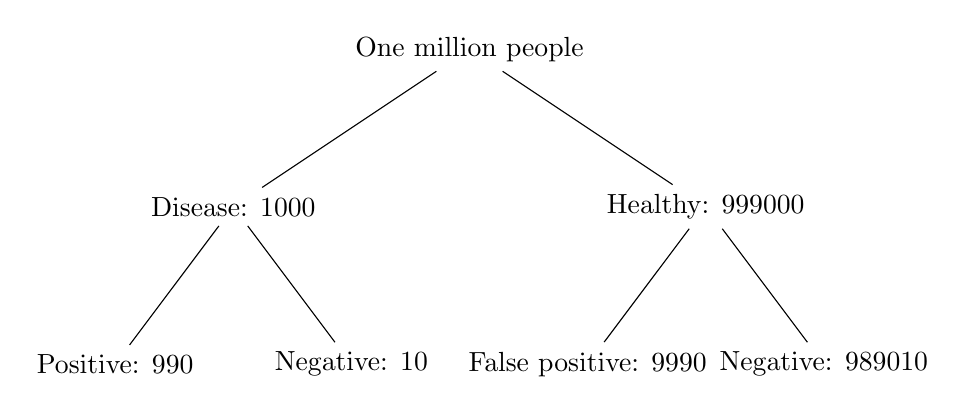
\begin{tikzpicture}[scale=1.0]
  \node (start) at (0,0) {One million people};
  \node (ill) at (-3,-2) {Disease: $1000$};
  \node (well) at (3,-2) {Healthy: $999000$};
  \node (illpos) at (-4.5,-4) {Positive: $990$};
  \node (illneg) at (-1.5,-4) {Negative: $10$};
  \node (wellpos) at (1.5,-4) {False positive: $9990$};
  \node (wellneg) at (4.5,-4) {Negative: $989010$};
  \draw (start) -- (ill);
  \draw (start) -- (well);
  \draw (ill) -- (illpos);
  \draw (ill) -- (illneg);
  \draw (well) -- (wellpos);
  \draw (well) -- (wellneg);
\end{tikzpicture}
\end{center}

The diagram reveals the secret: the false-positive fraction is small, but the healthy population is so large that false positives outnumber genuine cases ten to one. Intuition sees only $99\%$ test accuracy and forgets the prior information, prevalence. Bayes' entire spirit fits one sentence: \textbf{combine new evidence with the old background}. Prior probability $P(B_i)$ is the background, test result $A$ is new evidence, and $P(B_i\mid A)$ is the updated judgement. Medical screening, spam filtering, and search-engine spelling correction share this idea.

\section{What Can an Average Tell Us?}

Probability asks whether something happens; next ask what happens on average. A prize box contains $100$ tickets: $90$ say "Thanks for playing", prize $0$ yuan; $9$ pay $10$ yuan; $1$ pays $100$ yuan. How much does one draw yield on average?

Average does not mean a single result, which can only be $0$, $10$, or $100$. It means the total winnings across, say, ten thousand draws with replacement, divided by the number of draws. Probabilities predict about $9000$ prizes of $0$ yuan, $900$ of $10$, and $100$ of $100$, totalling roughly $9000\times 0+900\times 10+100\times 100=19000$ yuan, or $1.9$ per draw. In symbols,
\[
E=0\times 0.9+10\times 0.09+100\times 0.01=1.9\ (\text{yuan}).
\]

\begin{dingyi}
If a random quantity $X$ takes values $x_1,x_2,\dots,x_n$ with respective probabilities $p_1,p_2,\dots,p_n$, then
\[
E(X)=x_1p_1+x_2p_2+\cdots+x_np_n
\]
is the \textbf{mathematical expectation}, or mean, of $X$.
\end{dingyi}

Expectation is a probability-weighted average. One immediate consequence: if tickets cost $3$ yuan but expected prizes are $1.9$, long-term players lose an average $1.1$ yuan per game. Lotteries and casino games rest on this calculation: the house's expected gain is always positive and players' always negative. Expectation cannot predict the next game, but precisely predicts the long-term result.

The mean alone is insufficient. Two classes average $80$ marks; in one, everyone scores between $78$ and $82$, while in the other half get full marks and half fail. These are very different classes. We need a measure of fluctuation. Take each value's distance from the expectation, square it to prevent positive and negative deviations cancelling, then average with probability weights:
\[
\operatorname{Var}(X)=(x_1-E)^2p_1+(x_2-E)^2p_2+\cdots+(x_n-E)^2p_n,
\]
called \textbf{variance}. Large variance means spread-out, strongly fluctuating results; small variance means results cluster near the mean. The prize draw has large variance, with most leaving empty-handed and a few winning big; a die's outcome has much smaller variance. Investment's phrase "high risk, high return" translates mathematically as large expectation together with large variance.

\begin{fanli}
"The expected prize is $1.9$ yuan, so one ticket should give me about two yuan." Wrong: one draw pays only $0$, $10$, or $100$, never $1.9$. Expectation describes the long-run average, not the next result. Treating it as a single-trial prediction is a common misreading.
\end{fanli}

\section{Enough Throws Turn Disorder into Order}

We have repeatedly said that frequency stabilises near probability. Is this a law or merely common experience? Mathematicians made it a theorem.

\begin{dingli}[Law of large numbers, intuitive version]
Repeat a random experiment independently $n$ times under identical conditions, each result having expectation $E$. As $n$ grows, the arithmetic mean of the $n$ results approaches $E$ almost surely. With more trials, the probability of deviating from $E$ by more than any prescribed small amount approaches $0$.
\end{dingli}

A full proof needs more tools, but the idea is tangible: individual fluctuations cancel when averaged. Someone's exceptionally good luck offsets another's bad luck, leaving the expectation. This underpins insurance: nobody knows whether one customer will crash next year, but with a million customers total payouts become nearly deterministic, allowing premiums to be set precisely. Casinos likewise fear not one winning gambler, but too few gamblers. The law of large numbers is on their side.

An even more remarkable fact follows. One die has a flat distribution: $1$ through $6$ each occurs one-sixth of the time, six equal bars with no bell shape. With two dice, the sum $7$ has $6$ combinations, while $2$ and $12$ each have only $1$, giving a high centre and low ends. More dice make the sum's distribution approach a smooth symmetric bell. This is not peculiar to dice:

\begin{dingli}[Central limit theorem, intuitive version]
When many small independent random influences add together, whatever each influence's distribution, their sum or average approaches the same bell-shaped curve, the normal distribution. More influences give a closer approximation.
\end{dingli}

\begin{center}
\begin{tikzpicture}[scale=1.0]
  \draw[->] (-5,0) -- (5,0);
  \draw[->] (0,0) -- (0,3.2);
  \draw[smooth] plot coordinates {(-4.5,0.02) (-3.5,0.08) (-2.5,0.35) (-1.5,1.1) (-0.7,2.2) (0,2.8) (0.7,2.2) (1.5,1.1) (2.5,0.35) (3.5,0.08) (4.5,0.02)};
  \node at (0,-0.4) {$E$};
  \node at (4.6,-0.4) {Mean};
  \node at (0.9,3.0) {Count};
\end{tikzpicture}
\end{center}

This explains why heights, measurement errors, examination marks, and component dimensions all take similar bell shapes: each combines countless small influences. The central limit theorem is called probability's crown because it explains why diverse sources of disorder produce strikingly uniform order. Its proof is beyond this book; controlling precisely how quickly the approximation improves requires Chapter 12's analytic tools.

Having described order, we must confront a stubborn misconception. Roulette produces red seven times in succession; onlookers bet black, declaring it overdue. Wrong: the wheel has no memory, and the next red or black probability is unchanged. This \textbf{gambler's fallacy} mistakes long-run balance for short-run compensation. The law of large numbers says proportions approach balance after a hundred thousand trials, not that the next ten repay a debt. In 1913, a Monte Carlo casino reportedly produced black twenty-six times consecutively. Gamblers betting on overdue red lost piles of francs, all victims of this fallacy.

\begin{fanli}
"After five heads, tails is more likely next." Wrong: independent tosses leave the sixth-toss tail probability at $\dfrac{1}{2}$. What is rare is the entire six-head sequence, not a particular next step. Confusing a whole history's probability with the next outcome's probability drives the gambler's fallacy.
\end{fanli}

\begin{lianjie}
Chapter 9's limits return in new clothes: the law of large numbers says that the sequence of averages converges to the expectation, with a convergence notion allowing randomness. The central limit theorem's bell curve has equation $y=\dfrac{1}{\sqrt{2\pi}}e^{-x^2/2}$, containing both $\pi$ and $e$, one from circles and one from growth and compound interest. Circles, growth, and randomness meet in one formula. Mathematics has more hidden passageways than you might expect.
\end{lianjie}

\section{Finding Pi with Scattered Points}

So far, known probabilities predicted frequencies. Reverse that: use frequencies to calculate a deterministic constant seemingly unrelated to randomness. This is the Monte Carlo method, named after the casino city because random numbers fuel it.

Take a square sheet of side $2$ and draw an inscribed circle of radius $1$. The square's area is $4$, the circle's $\pi$. Scatter points randomly into the square, perhaps sesame seeds or blind pencil marks. Suppose $N$ points are placed and $M$ fall inside the circle. If every position in the square is equally likely,
\[
\frac{M}{N}\approx \frac{\text{Circle area}}{\text{Square area}}=\frac{\pi}{4},
\qquad\text{so}\qquad
\pi\approx \frac{4M}{N}.
\]

\begin{center}
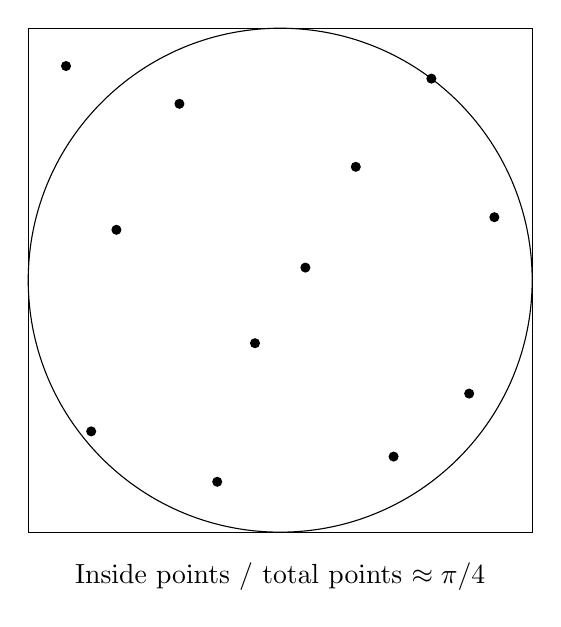
\begin{tikzpicture}[scale=1.6]
  \draw (0,0) rectangle (4,4);
  \draw (2,2) circle (2);
  \fill (0.5,0.8) circle (0.04);
  \fill (1.2,3.4) circle (0.04);
  \fill (2.6,2.9) circle (0.04);
  \fill (3.5,1.1) circle (0.04);
  \fill (1.8,1.5) circle (0.04);
  \fill (2.9,0.6) circle (0.04);
  \fill (0.7,2.4) circle (0.04);
  \fill (3.2,3.6) circle (0.04);
  \fill (2.2,2.1) circle (0.04);
  \fill (1.5,0.4) circle (0.04);
  \fill (3.7,2.5) circle (0.04);
  \fill (0.3,3.7) circle (0.04);
  \node at (2,-0.35) {Inside points / total points $\approx \pi/4$};
\end{tikzpicture}
\end{center}

The method is charmingly crude: a few hundred points might give $\pi\approx 3.1$; hundreds of thousands, scattered by computer, can reach two or three decimal places. Accuracy improves slowly: error is roughly inversely proportional to $\sqrt{N}$, so tenfold improvement needs a hundred times as many points. It is not the fastest way to estimate $\pi$. Its real strength is measuring bizarrely shaped regions with no area formula, or volumes in high dimensions. Simulating particles passing through matter, pricing complex financial products, and rendering light in computer graphics all share the trick: \textbf{probe otherwise inaccessible quantities through random experiments}. Chapter 11's integration returns unexpectedly: Monte Carlo is essentially integrating by throwing dice.

An older version is Buffon's needle. Randomly drop needles of length $l$ onto parallel lines spaced $d$ apart, with $l\le d$. In the eighteenth century, Buffon proved that the probability of crossing a line is exactly $\dfrac{2l}{\pi d}$. Repeatedly drop needles and measure the crossing frequency $f$ to infer
\[
\pi\approx \frac{2l}{fd}.
\]
A needle, paper, and a quiet afternoon let pi emerge from random noise. The proof uses integration: both position and angle are random, and weighting all positions by their chances turns the crossing condition into an integrable region. Details belong to further climbing.

\begin{shiyan}
\textbf{Estimating $\pi$ by scattering points at home.} Draw a $10\times 10$ square on squared paper. Using one corner as centre and the side length as radius, draw a quarter-circle with compasses. Close your eyes and make random pencil marks, opening them after each to record whether the point lies inside or outside the quarter-circle; redo marks outside the paper. After $100$ marks, with $M$ inside, estimate $\pi$ by $\dfrac{4M}{100}$. Combine classmates' results: pool five people's $500$ points and compare accuracy before and after pooling. Watch the law of large numbers at work: more points give a steadier estimate.
\end{shiyan}

\begin{toolbox}
New tools from this chapter:
\begin{itemize}
  \item \textbf{Complementary calculation}: For at least one occurrence, calculate none and subtract from $1$.
  \item \textbf{Conditional probability and Bayes' formula}: $P(A\mid B)=\dfrac{P(A\text{ and }B)}{P(B)}$; combine new evidence with prior background.
  \item \textbf{Checking independence}: Require $P(A\text{ and }B)=P(A)P(B)$, not an intuitive impression.
  \item \textbf{Expectation and variance}: $E(X)$ describes long-term averages; $\operatorname{Var}(X)$ describes fluctuation.
  \item \textbf{Law of large numbers}: With enough trials, averages approach expectations; this concerns the long run, not the next game.
  \item \textbf{Monte Carlo methods}: Approximate areas, constants, and integrals through random-trial frequencies.
\end{itemize}
\end{toolbox}

\section{When Statistics Starts to Mislead}

Learning the tools also means recognising traps. Beyond birthdays and the gambler's fallacy, several mechanisms particularly catch the half-informed.

First is survivorship bias. During the Second World War, statisticians studied bullet holes in returning bombers. Wings had the most holes, so officers proposed reinforcing them. Mathematicians instead recommended the engines, which showed few holes: aircraft hit there never returned. The visible sample contained only survivors and was inherently incomplete. Arguments that education is useless, citing a few wealthy dropouts, and success courses interviewing only surviving companies make the same mistake.

Second is the illusion of averages. A company's average annual salary of five hundred thousand yuan might combine a boss earning fifty million with everyone else near fifty thousand. Expectations are sensitive to extremes; the median, the middle ranked value, may be more honest. Whenever you see an average, ask which kind, and whose values were averaged.

Third is mistaking correlation for causation. Ice-cream sales and drownings rise together: does ice cream cause drowning? Summer is the common cause. Two rising quantities may have a causal relationship in either direction, a shared third cause, or only coincidence. Statistics detects associations; establishing causality needs controlled experiments or deeper mechanisms. Every citizen in the data age needs this lesson.

\begin{pandeng}
Further keywords await: \textbf{normal distribution}, its exact bell-curve equation and the $3\sigma$ rule; \textbf{hypothesis testing}, judging quantitatively whether a difference is chance or a genuine effect; \textbf{rigorous laws of large numbers}, entered through Chebyshev's inequality; \textbf{Markov chains}, random processes where tomorrow depends only on today, powering web ranking; and \textbf{information theory}, measuring surprise probabilistically in bits. School courses and competitions also offer elegant probability recurrences, including the famous gambler's ruin problem.
\end{pandeng}

\section*{Questions to Think About}

\textbf{Observation}

1. Shuffle a deck, turn over cards, and record whether the first two share a suit. Repeat twenty times and estimate the frequency. Then calculate the theoretical probability and compare. Hint: the first card is arbitrary; the second's matching probability depends on how many cards of that suit remain.

2. Collect a week's household electricity usage from differences in meter readings. Calculate the mean, then consider what factor could make one day differ most from it. Is that a source of variance?

\textbf{Proof}

1. Prove that if $A$ and $B$ are independent, then not $A$ and not $B$ are independent too. Hint: use $P(A\text{ does not occur})=1-P(A)$ to expand $P(\text{neither occurs})=1-P(A)-P(B)+P(A)P(B)$, then factorise.

2. Rephrase the birthday problem: how many people make the probability of at least one match exceed $99\%$? Show your estimation. Hint: exact solution is unnecessary; try all-different probabilities for $40$, $50$, and $60$ people using logarithms or successive products.

\textbf{Challenge}

1. The Monty Hall problem: three doors hide a car and two goats. After you choose a door, the host, who knows the answer, opens another door revealing a goat and offers a switch. What is the probability of winning by switching? Justify by conditional probability or enumeration, and explain why two remaining doors do not mean equal one-half chances. Hint: the host does not open a random door; the action carries information.

2. Design a Monte Carlo experiment estimating $\sqrt{2}$ using only scattered points and area comparisons. Hint: $\sqrt{2}$ is a side or diagonal length of a simple figure; alternatively consider areas near $y=x^2$.

\section*{The Door to the Next Chapter}

At several crucial moments we said to scatter hundreds of thousands of points, toss a hundred thousand times, or repeat an enormous number of trials. Mathematics supplies formulas, but who performs those dreary repetitions? Hands cannot keep up and minds make mistakes. One machine, however, loves this work: it can throw billions of dice per second without tiring or complaining.

Monte Carlo truly changed the world after electronic computers arrived. Among the earliest tasks for the first general-purpose electronic computer was simulating neutrons travelling through matter with random numbers. New questions immediately followed: if a computer's random numbers come from deterministic formulas, are they truly random? Which problems can it simulate in an instant, and which remain unfinished after ten thousand years? Next chapter opens the door between mathematics and computing.
